\subsection{Опис графічного інтерфейсу та взаємодії з користувачем}

Для забезпечення зручної взаємодії користувача з розробленими алгоритмами масштабування було створено графічний інтерфейс. Головне вікно програми спроєктовано таким чином, щоб надати швидкий доступ до всіх параметрів трансформації та максимізувати площу для візуального аналізу результатів (рис.~\ref{fig:main_window}).

\begin{figure}[htbp]
	\centering
	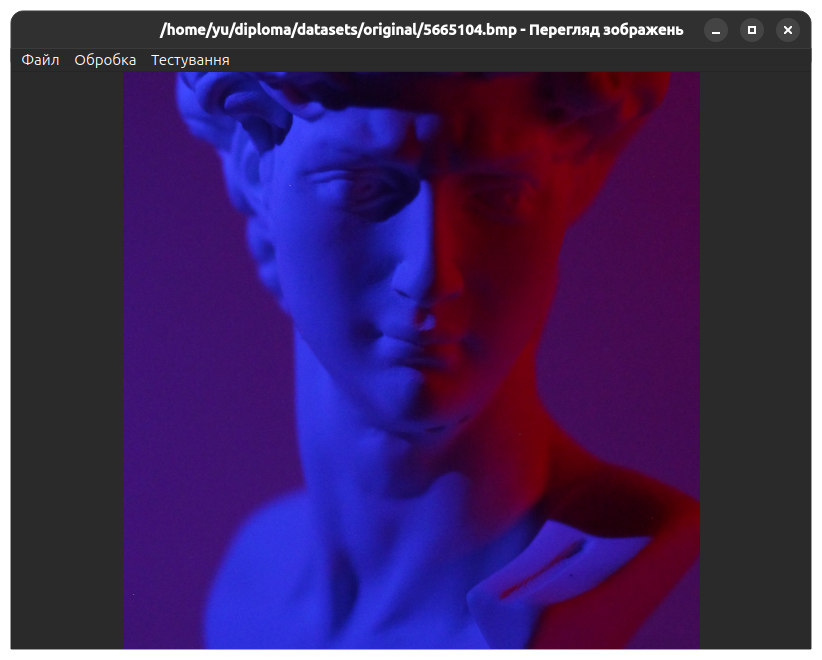
\includegraphics[width=0.8\textwidth]{figures/mainwindow}
	\caption{Головне вікно розробленої програми}
	\label{fig:main_window}
\end{figure}

\newpage
У верхній частині вікна розташоване головне меню (\textit{Menu Bar}). Воно відповідає за базові операції роботи з файлами: завантаження вихідного зображення для обробки та збереження отриманого результату на диск. Окрім стандартних файлових операцій, через головне меню здійснюється виклик спеціалізованого діалогового вікна автоматизованого тестування. Воно використовується для пакетного прогону алгоритмів та збору метрик продуктивності без відображення проміжних графічних результатів.

Програма підтримує два сценарії взаємодії з вхідними даними. Користувач може застосувати обраний алгоритм інтерполяції до всього зображення цілком або ж виділити мишею специфічну прямокутну область (\textit{Region of Interest, ROI}) безпосередньо у вікні перегляду. Другий режим є особливо корисним для детального аналізу роботи алгоритмів на складних ділянках, таких як різкі переходи кольорів або дрібні текстури, без необхідності витрачати обчислювальні ресурси на обробку всього масиву пікселів. Візуальне порівняння цих двох підходів наведено на рис.~\ref{fig:process_whole_image} та рис.~\ref{fig:process_selected_area}.

\begin{figure}[htbp]
	\centering
	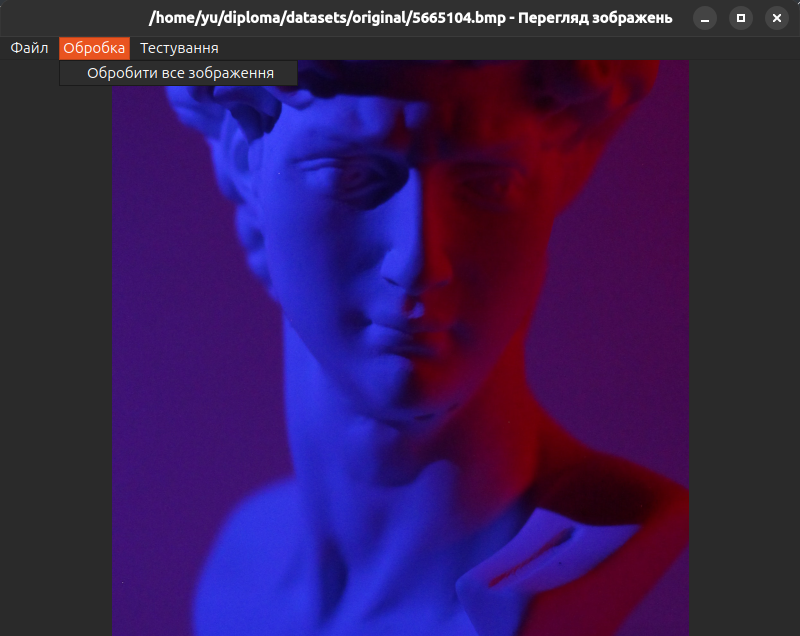
\includegraphics[width=0.75\textwidth]{figures/processWholeImage}
	\caption{Режим масштабування всього зображення}
	\label{fig:process_whole_image}
\end{figure}

\begin{figure}[htbp]
	\centering
	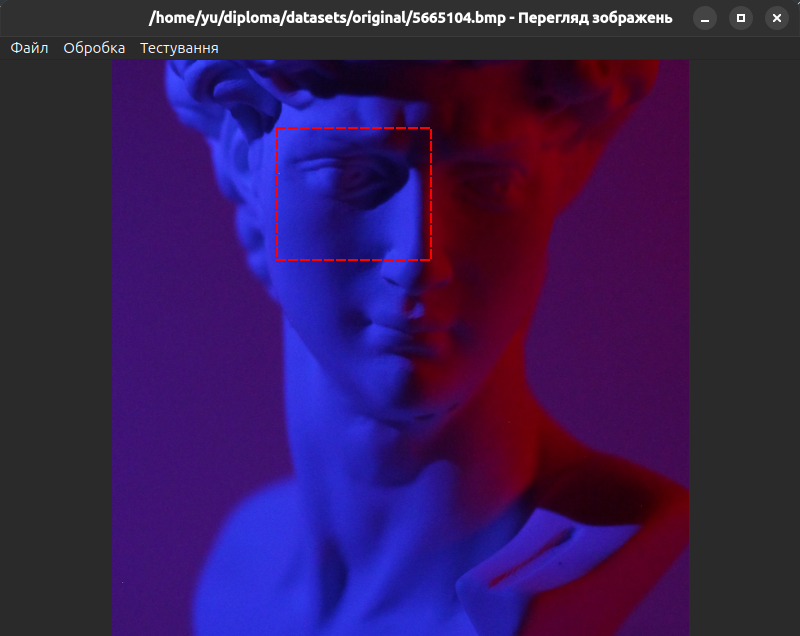
\includegraphics[width=0.75\textwidth]{figures/processSelectedArea}
	\caption{Режим масштабування виділеної області}
	\label{fig:process_selected_area}
\end{figure}

\newpage
Варто зазначити, що незалежно від обраного сценарію просторової обробки, вибір конкретного математичного методу масштабування здійснюється через випадне меню (\textit{Drop-down menu}), розташоване на панелі налаштувань. Воно містить інтегрований перелік усіх доступних алгоритмів, включаючи як базові індустріальні методи, так і розроблені барицентричні підходи (рис.~\ref{fig:method_selection_menu}).

\begin{figure}[htbp]
	\centering
	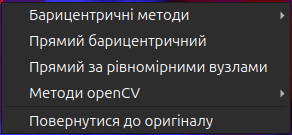
\includegraphics[width=0.6\textwidth]{figures/methodsMenu} 
	\caption{Випадне меню вибору алгоритму інтерполяції}
	\label{fig:method_selection_menu}
\end{figure}

Після вибору алгоритму інтерполяції програма ініціює наступний етап налаштування, виводячи на екран діалогове вікно конфігурації геометричного перетворення. У цьому вікні користувачу необхідно задати два ключові параметри: числовий коефіцієнт масштабування та напрямок трансформації. Вибір напрямку реалізовано у вигляді перемикача між режимами збільшення (\textit{Upscaling}) та зменшення (\textit{Downscaling}) зображення. Такий явний поділ є важливим, оскільки внутрішня логіка розрахунку кроку дискретизації та формування цільової матриці суттєво відрізняється для цих двох операцій (рис.~\ref{fig:scale_config_window}).

\begin{figure}[htbp]
	\centering
	\begin{minipage}{0.48\textwidth}
		\centering
		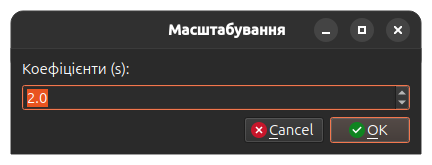
\includegraphics[width=\linewidth]{figures/coeficents}
		\caption*{а) Введення коефіцієнта масштабування}
	\end{minipage}\hfill
	\begin{minipage}{0.48\textwidth}
		\centering
		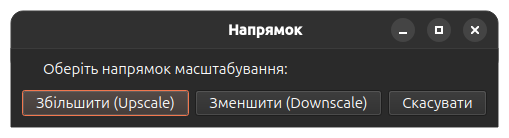
\includegraphics[width=\linewidth]{figures/direction}
		\caption*{б) Вибір напрямку (\textit{Upscaling}/\textit{Downscaling})}
	\end{minipage}
	\caption{Налаштування параметрів геометричного перетворення}
	\label{fig:scale_config_window}
\end{figure}

Особливістю розробленого графічного інтерфейсу є його адаптивність до специфіки обраного математичного апарату. Якщо користувач обирає з меню локальний барицентричний метод, логіка конфігурації автоматично розширюється, і на екран виводиться додаткове діалогове вікно для налаштування параметра $K$ (рис.~\ref{fig:local_k_window}). 

\begin{figure}[htbp]
	\centering
	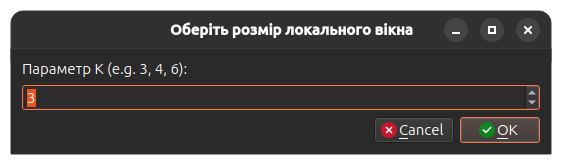
\includegraphics[width=0.8\textwidth]{figures/localSize}
	\caption{Додаткове вікно введення параметра $K$ для локального барицентричного методу}
	\label{fig:local_k_window}
\end{figure}

Цей параметр є унікальним для локального підходу: він визначає розмір розрахункового вікна (околу), тобто фіксовану кількість сусідніх вузлів інтерполяції, які будуть враховуватися при обчисленні ваг для кожного цільового пікселя. Надання користувачу можливості ручного керування параметром $K$ через графічний інтерфейс є критично важливим архітектурним рішенням. Воно дозволяє гнучко балансувати між швидкодією алгоритму (при виборі малих значень $K$) та точністю наближення функції інтенсивності на ділянках зі складною текстурою (що досягається при збільшенні розміру околу).